\begin{appendix}

\lstset{basicstyle=\small\ttfamily}

\section{\name Full Query Interface}
\label{sec:fullquery}
In this section, we list the full query interface for spatial operations and index
management in SQL query language and DataFrame API of \name.

\subsection{SQL Query Language}
\Paragraph{Points.} Users can use keyword \texttt{POINT} followed by a list of
expressions to express multi-dimensional points, where the number of expressions
indicates the number of dimensions. For example, we can use \texttt{Point(x - 1, y * 2)}
to express a two dimensional point with the value of $x - 1$ as the first dimension
and the value of $y * 2$ as the second dimension.

\Paragraph{Range predicates.} \name supports two different kinds of range queries:
box range queries and circle range queries. For box range queries, users should
use the following predicate to check if points are in the specific bounding box:
\begin{lstlisting}[language=SQL]
p IN RANGE(low, high)
\end{lstlisting}
In the predicate above, parameters \texttt{p}, \texttt{low} and \texttt{high}
should be point objects expressed by the grammar for points described above.
Specifically, \texttt{p} indicates the input point for predicate checking, while
\texttt{low} and \texttt{high} specify the bounding box.

Similarly, for circle range queries, users should use predicates as below:
\begin{lstlisting}[language=SQL]
p IN CIRCLERANGE(c, rd)
\end{lstlisting}
Note that \texttt{p} is the same as box range queries, while the point object
\texttt{c} and the constant \texttt{rd} indicates a circle centered at point
\texttt{c} with radius \texttt{rd} as the predicate area.

\Paragraph{$k$NN predicates.} Similar to range predicates, \name provides $k$NN
predicates as following:
\begin{lstlisting}[language=SQL]
p IN KNN(q, k)
\end{lstlisting}
It checks if \texttt{p} is in the $k$NN of point $q$ within the selection
domain. The selection domain is indicated by the relation after the same
level \texttt{WHERE} clause (when $k$NN predicates work as select conditions),
or the right-hand side relation of a $k$NN join operation (when $k$NN predicates
work as join conditions).

\Paragraph{Distance joins.} Users can use the SQL statement below to
express a distance join between two tables \texttt{R} and \texttt{S} with
distance threshold \texttt{rd}:
\begin{lstlisting}[language=SQL]
R DISTANCE JOIN S ON s IN CIRCLERANGE(r, rd)
\end{lstlisting}
Note that point \texttt{s} (resp. \texttt{r}) should be built from a record in
table $S$ (resp. $R$), or \name will be unable to resolve it.

\Paragraph{$k$NN joins.} A $k$NN join between table \texttt{R} and table \texttt{S}
can be expressed as following SQL statement:
\begin{lstlisting}[language=SQL]
R KNN JOIN S ON s IN KNN(r, k)
\end{lstlisting}
Similar to distance joins, $s$ (resp. $r$) should be built from a record in \texttt{S}
(resp. \texttt{R}). Users can also invoke an approximate $k$NN join using ZKJSpark
by replacing \texttt{KNN JOIN} by \texttt{ZKNN JOIN}.

\Paragraph{Index management.} \name allows users to manipulate indexes
easily with index management commands. Specifically, we can create
an index with the following command:
\begin{lstlisting}[language=SQL]
CREATE INDEX idx_name ON R(x, ...) USE idx_type
\end{lstlisting}
It builds a new index over a set of attributes in table \texttt{R} using the specific index
type (which can be R-tree, tree map or hash map), and names it as \texttt{idx\_name}.
We can check the built index on table \texttt{R} anytime using:
\begin{lstlisting}[language=SQL]
SHOW INDEX ON R
\end{lstlisting}
In addition, users can drop indexes by index names and/or table names using:
\begin{lstlisting}[language=SQL]
DROP INDEX idx_name ON table_name
DROP INDEX table_name
\end{lstlisting}

\subsection{DataFrame API}
\lstset{basicstyle=\scriptsize\ttfamily}
\Paragraph{Points.} We introduce point objects in DataFrame API, which wrap a list
of expressions into a multi-dimensional point that can be processed in \name. For
example, we can express a three dimensional point as following:
\begin{lstlisting}[language=java]
Point(tb("x"), tb("y"), tb("z"))
\end{lstlisting}
Specifically, the code above wraps three attributes \texttt{x}, \texttt{y} and \texttt{z}
from table \texttt{tb} into a point object for further processing.

\Paragraph{Single-relation operations.} Users can apply (box or circle) range queries
and $k$NN queries directly on data frames. Specifically, in DataFrame API, \name provides
following functions:
\begin{lstlisting}[language=java]
range(base: Point, low: Point, high: Point)
circleRange(base: Point, center: Point, r: Double)
knn(base: Point, q: Point, k: Int)
\end{lstlisting}
In the APIs described above, \texttt{base} indicates the point objects to be filtered,
while the other parameters give filter conditions.

\Paragraph{Join operaitons.} In the DataFrame API of \name, distance joins
and $k$NN joins can be expressed with following functions:
\begin{lstlisting}[language=java]
distanceJoin(other: DataFrame, left_key: Point,
             right_key: Point, rd: Double)
knnJoin(other: DataFrame, left_key: Point,
        right_key: Point, k: Int)
\end{lstlisting}
These functions will join the current data frame with another data frame \texttt{other}
on join conditions over \texttt{left\_key} and \texttt{right\_key}.

\Paragraph{Index management.} Users can easily create and drop indexes on data
frames with functions below:
\begin{lstlisting}[language=java]
index(index_type: IndexType, index_name: String, 
      attrs: Seq[Attribute])
dropIndex()
\end{lstlisting}

\setcounter{theorem}{0}
\section{Proof of Theorem 1}
\label{sec:proof1}
\begin{theorem}
For any partition $R_i$ where $i \in[1, n]$, we have:
\[\forall r \in R_i, \knn(r, S) \subset \{s|s \in S, |cr_i, s| \leq
\gamma_i\}, \textrm{ for }\gamma_i \textrm{ defined in
}\eqref{eq:rkjbound}.\]
\end{theorem}
\begin{proof}
Recall that $\knn(cr_i, S')=\{s_1, \ldots, s_k\}$ (in ascending
order of their distances to $cr_i$), and $u_i=\max_{r\in R_i}|r,
cr_i|$. Hence, for any $r \in R_i$, and for any $t \in [1, k]$, we
have:
\begin{align*}
|r, s_t|& \leq |r, cr_i| + |cr_i, s_t| \quad \textrm{(triangle inequality)}\\
   &\leq u_i + |cr_i, s_k|. \quad \textrm{(by construction)}
\end{align*}
This implies that a circle centered at $r$ with radius $(u_i + |cr_i,
s_k|)$ will cover at least $k$ points (i.e., at least $s_1, s_2, s_3,
.. s_k$) in $S'\subset S$. In other words, $\knn(r, S) \subset
S_r=\{s|s \in S, |r, s| \leq u_i + |cr_i, s_k|\}$. We denote this set
as the {\em cover set} of record $r$.

For each element $e \in S_r$, we have:
\begin{align*}
  |e, cr_i| & \leq |e, r| + |r, cr_i| \quad (\forall r\in R_i \textrm{, triangle inequality)} \\
  & \leq u_i + |cr_i, s_k| + u_i \\
  & = \gamma_i,
\end{align*}
 which implies $S_r$ is a subset
of $\{s|s \in S, |cr_i, s| \leq \gamma_i\}$.  Thus, $\forall r \in
R_i, \knn(r, S) \subset S_r \subset \{s|s \in S, |cr_i, s| \leq
\gamma_i\}.$
\end{proof}

\section{Additional Experiments}
\label{sec:addexp}
In this section, we show additional experiment results on how partition size influence
the performance of table indexing and different spatial operations in \name. Besides,
we present the influence of dimensionality on RC data sets for range and $k$NN queries
as well. 

\begin{figure}[!h]
	\centering
	% 	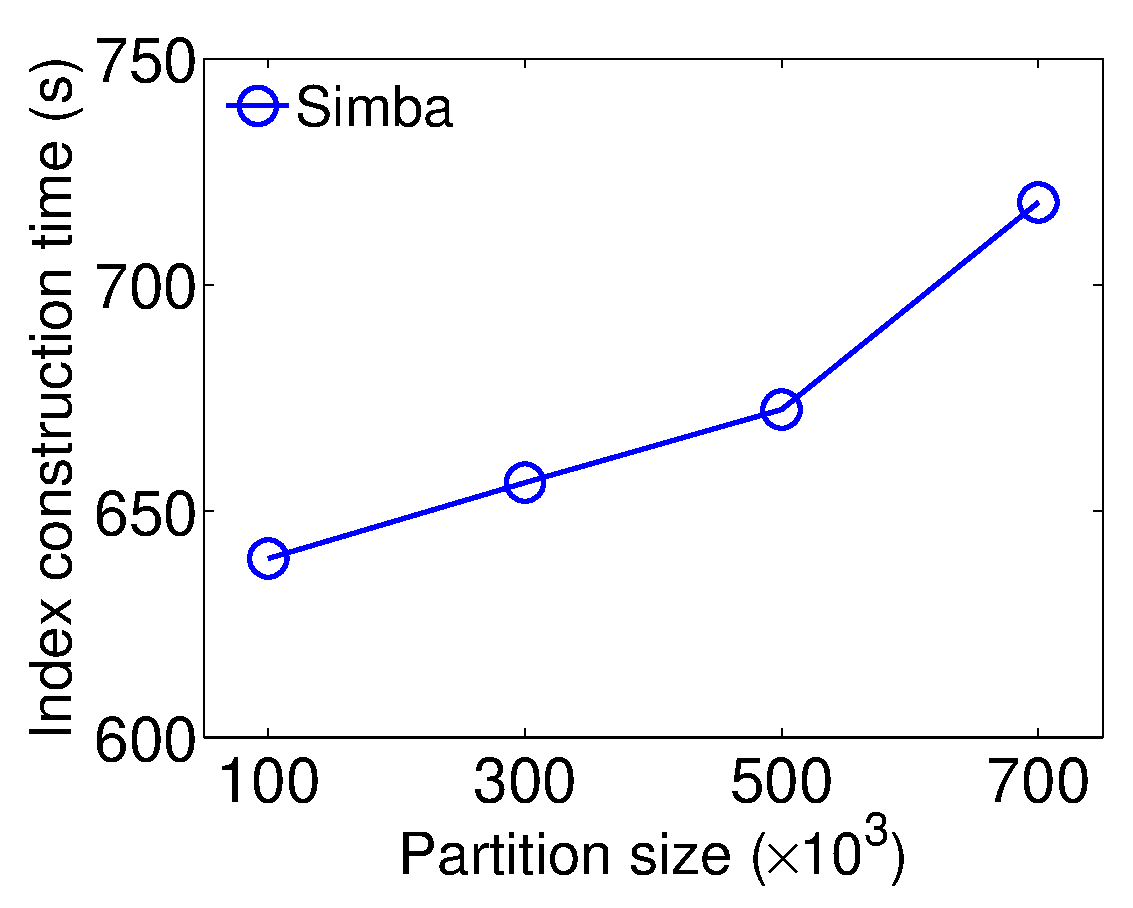
\includegraphics[width=1.55in]{figs/exp/osm_index_partsize_time}
	% 	\label{fig:index_partsize}}
	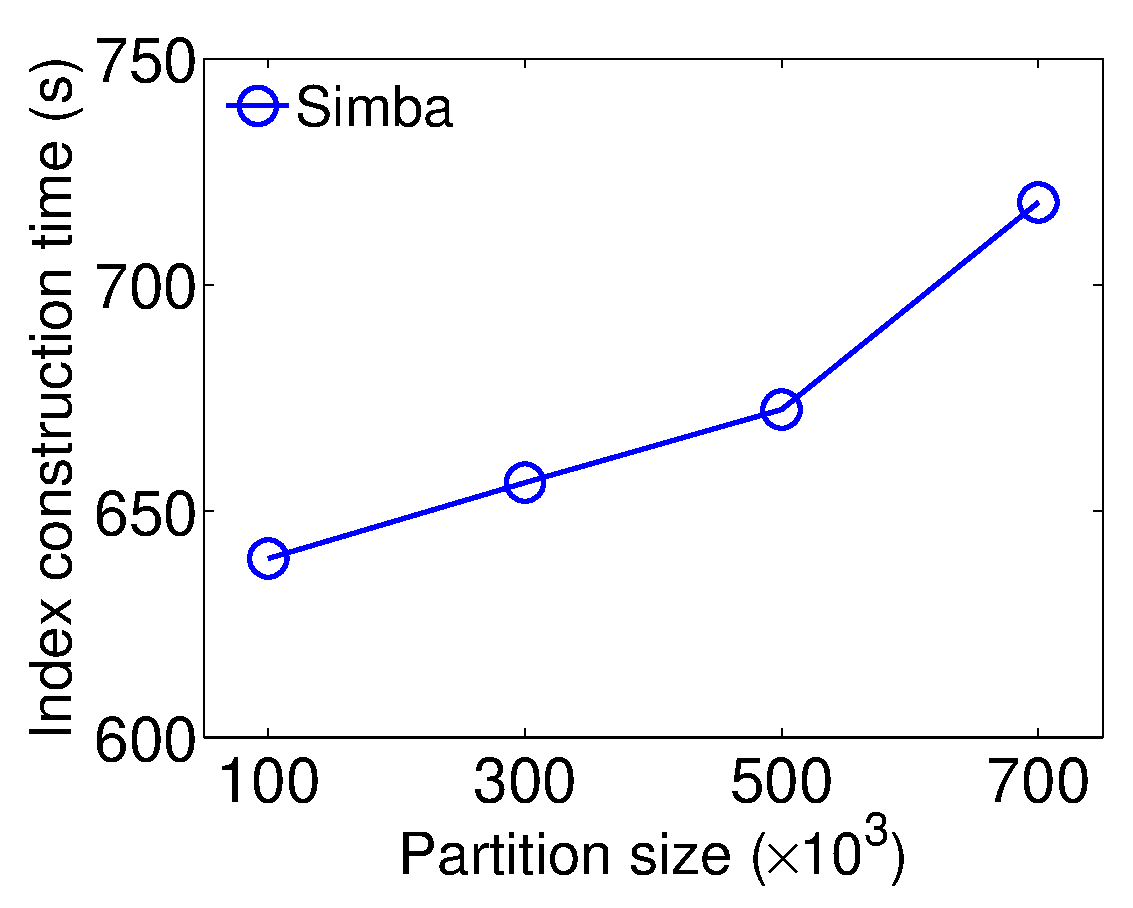
\includegraphics[width = 1.74in]{figs/exp/osm_index_partsize_time}\vspace{-4mm}
	\caption{Index construction cost: effect of partition size.}
	\label{fig:index_partsize}\vspace{-1mm}
\end{figure}

Figure \ref{fig:index_partsize} shows that its index construction cost
grows roughly linearly with respect to (wrt) partition size. This is
because it is more costly to build local indexes over larger
partitions (which outweighs the savings resulted from processing less
number of partitions). % Note that We only show results for
% \name since expected partition sizes for other systems are fixed to
% the HDFS block size.

\begin{figure}[!h]
	\centering
	\subfigure[Effect of partition size (number of records per partition).]{
		\label{fig:osm_rect_partsize}
		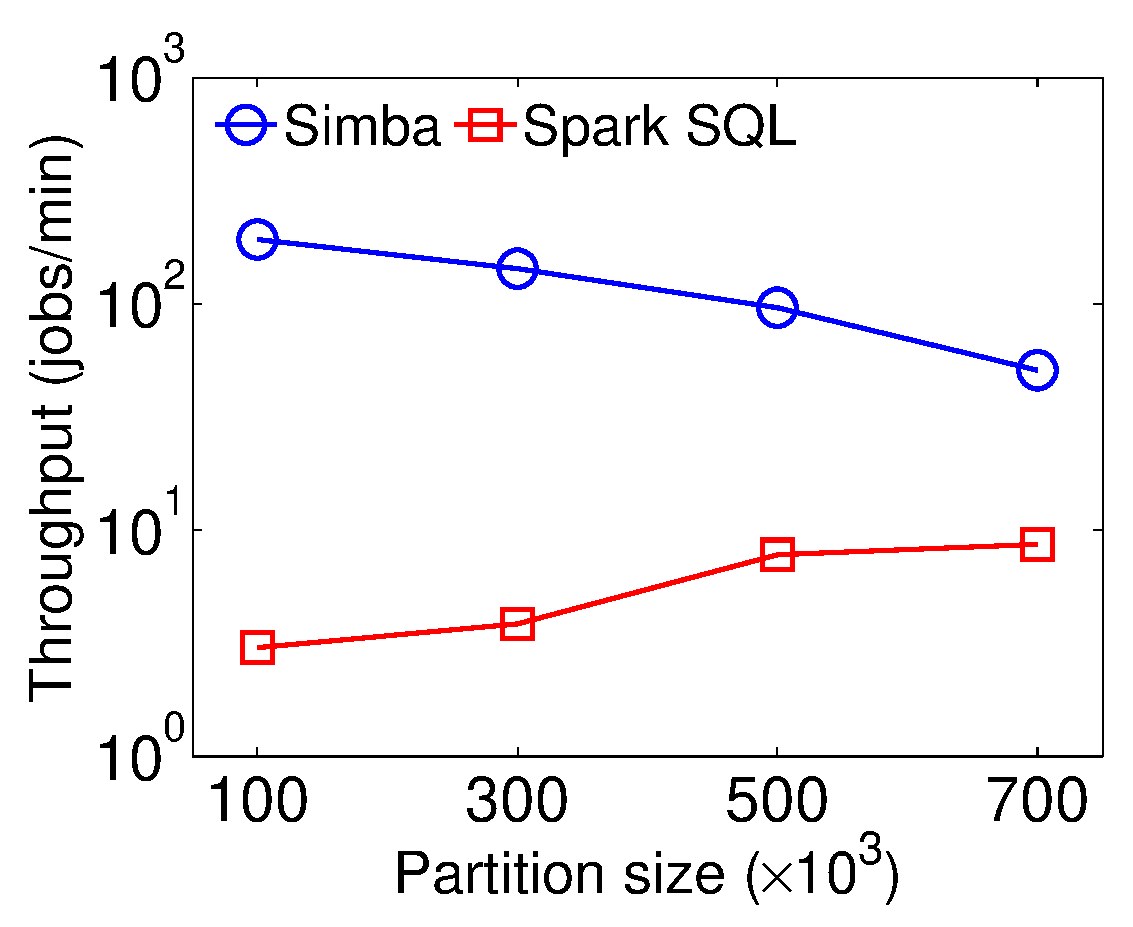
\includegraphics[width=1.55in]{figs/exp/osm_rect_partsize_throughput}
		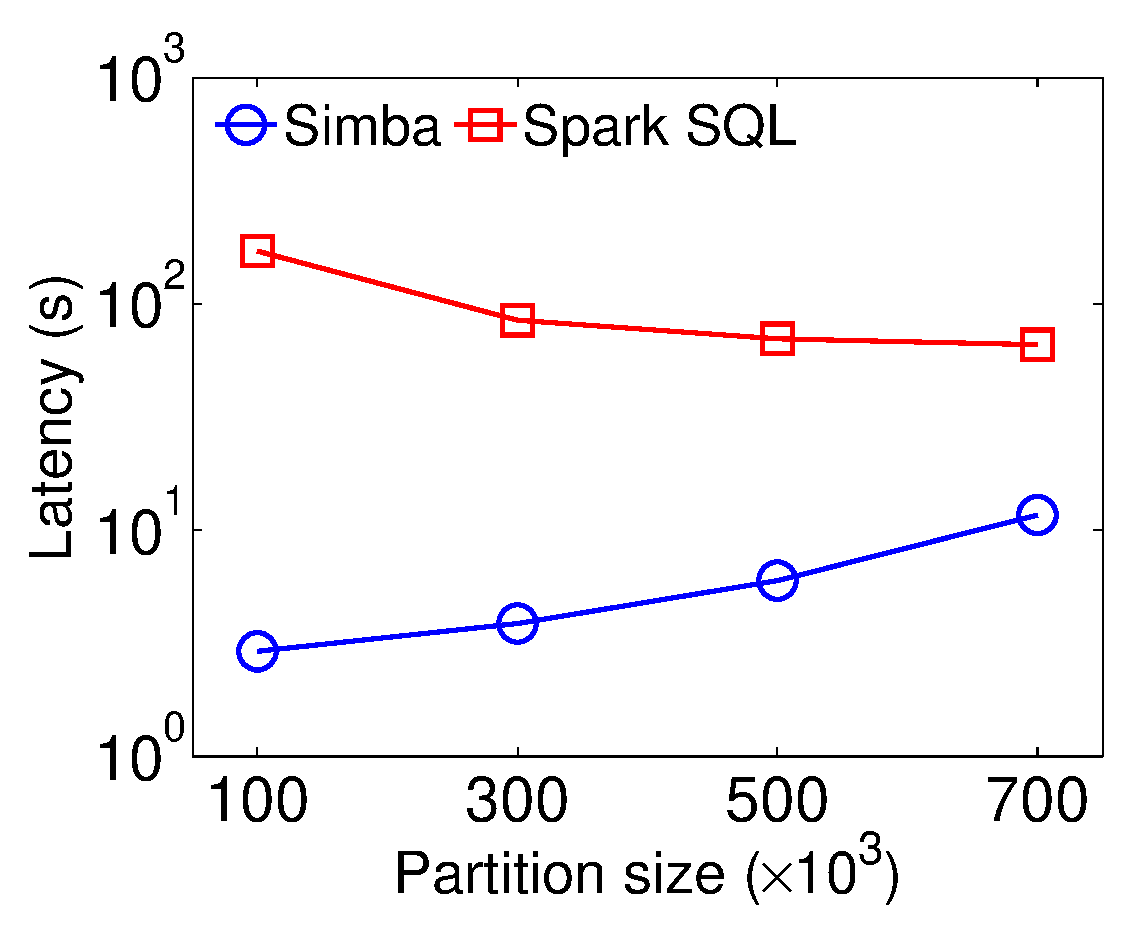
\includegraphics[width=1.55in]{figs/exp/osm_rect_partsize_latency}
	}
	\caption{Range query performance on OSM: partition size.}
	\label{fig:rangepartition}\vspace{-1mm}
\end{figure}

Figure \ref{fig:rangepartition} shows the effect of partition size
(from $1 \times 10^5$ to $7 \times 10^5$ records per partition). As it
increases, the pruning power of global index in \name shrinks and so
does \name's performance. On the other hand, Spark SQL's performance
slightly increases as it requires fewer partitions to
process. Nevertheless, \name is still much more efficient due to its
local indexes and spatial query optimizer.

\begin{figure}[!h]
	\centering
	\subfigure[Effect of partition size (number of records per partition).]{
		\label{fig:osm_knn_partsize}
		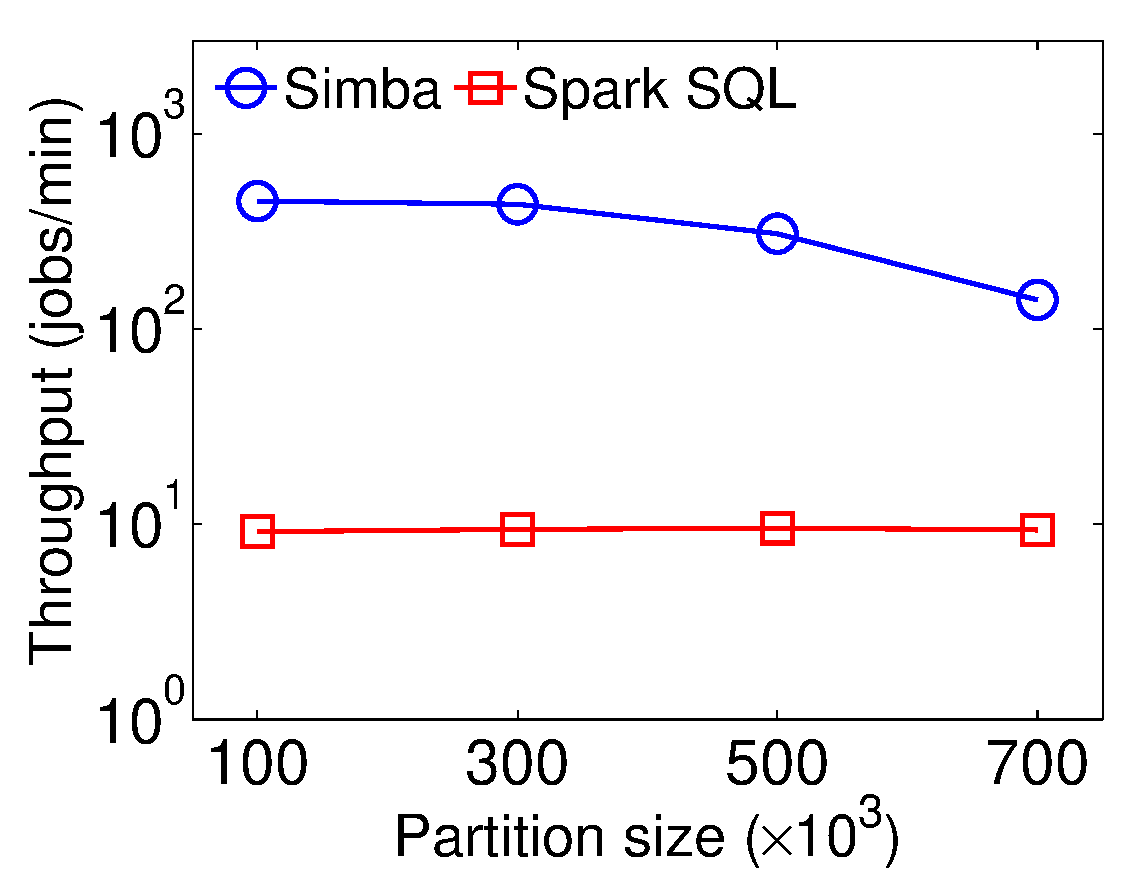
\includegraphics[width=1.55in]{figs/exp/osm_knn_partsize_throughput}
		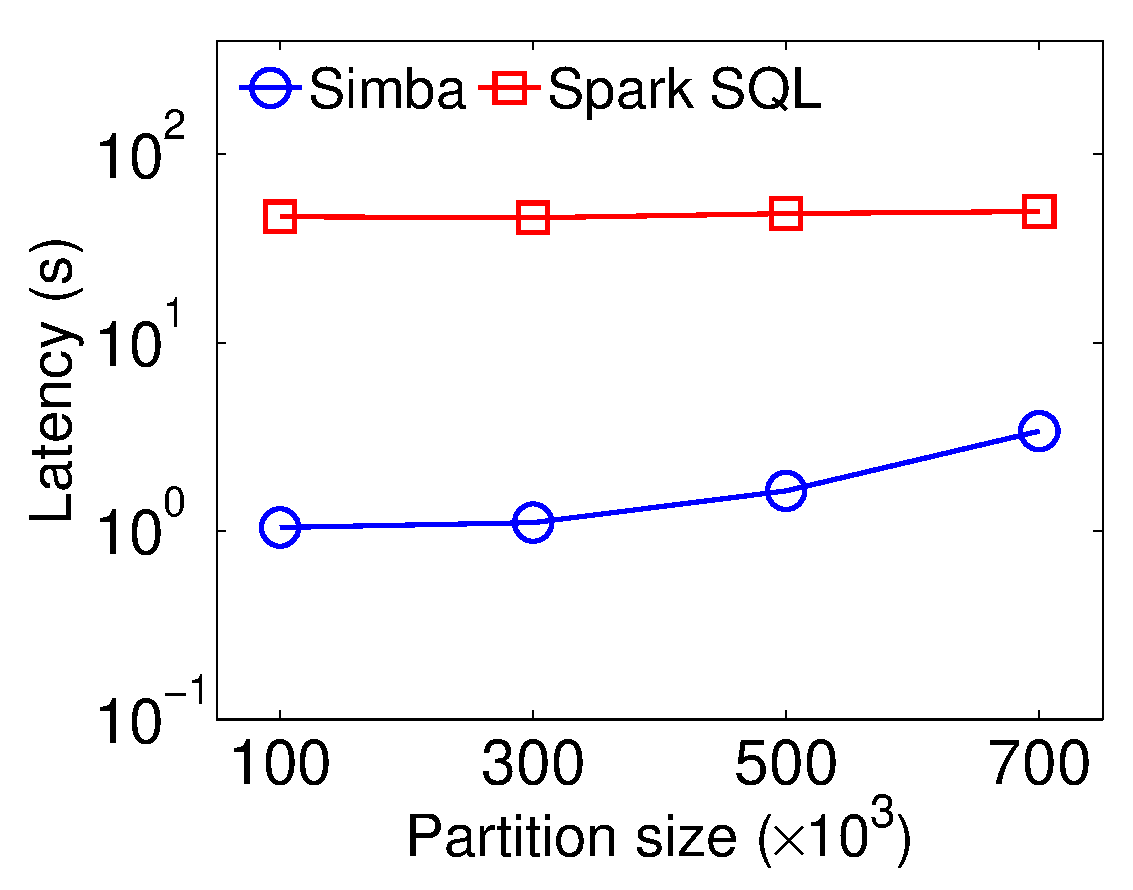
\includegraphics[width=1.55in]{figs/exp/osm_knn_partsize_latency}
	}\vspace{0mm}
	\caption{$k$NN query performance on OSM: partition size.}\vspace{-1mm}
	\label{fig:knnparition}
\end{figure}

In Figure \ref{fig:knnparition}, as the partition size increases,
the performance of \name decreases as the pruning power of global
index will drop when the partitions become larger.

Figure \ref{fig:osm_disj_partsize} shows the effect of partition size
on different distance join algorithms. As the partition size grows,
the running time of DJSpark and HDJSpark increases slightly, as the
pruning power of global join phase reduces when the partition
granularity is decreasing.  In contrast, BDJSpark-R becomes faster
because fewer local join tasks are required in the algorithm.

\begin{figure}[!h]
  \subfigure[Distance Join]{
		\label{fig:osm_disj_partsize}
		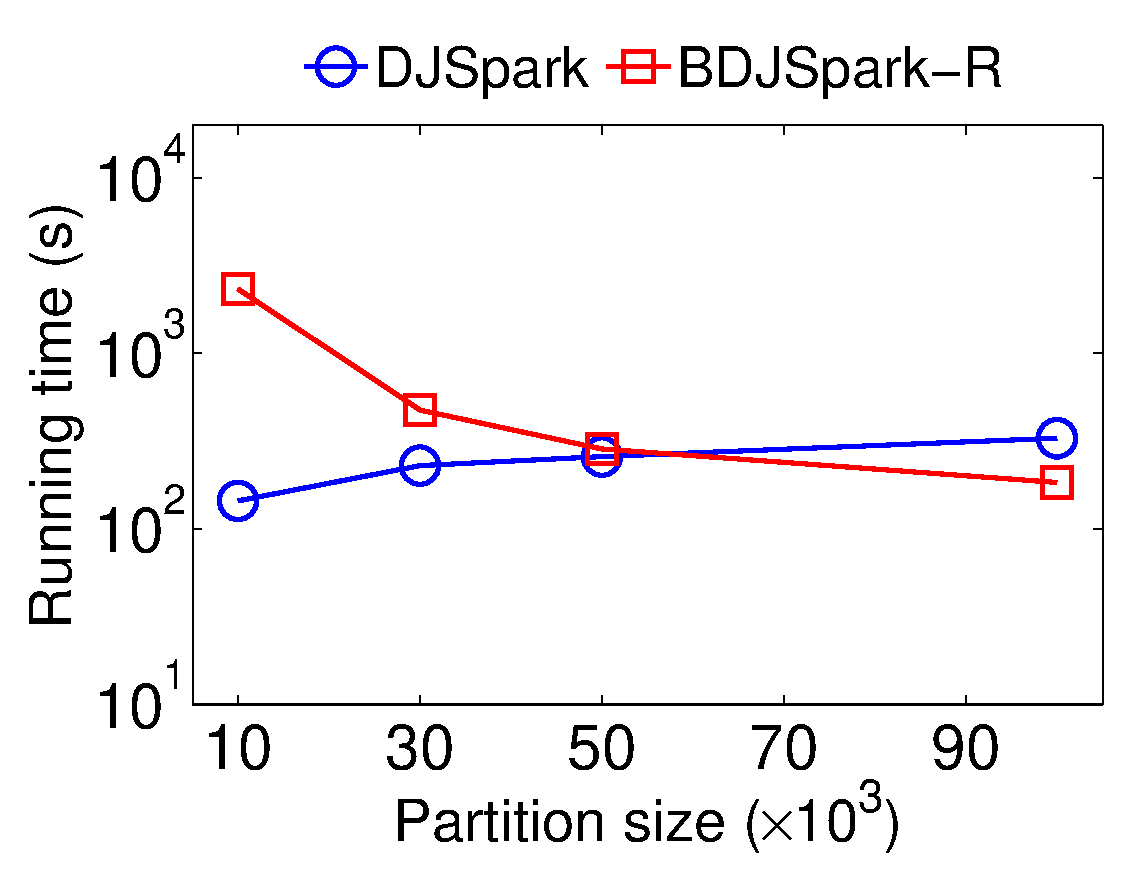
\includegraphics[width=1.55in]{figs/exp/osm_disj_partsize}
	} %\vspace{-6mm}
  \subfigure[$k$NN Join]{
    \label{fig:osm_knnj_partsize}
    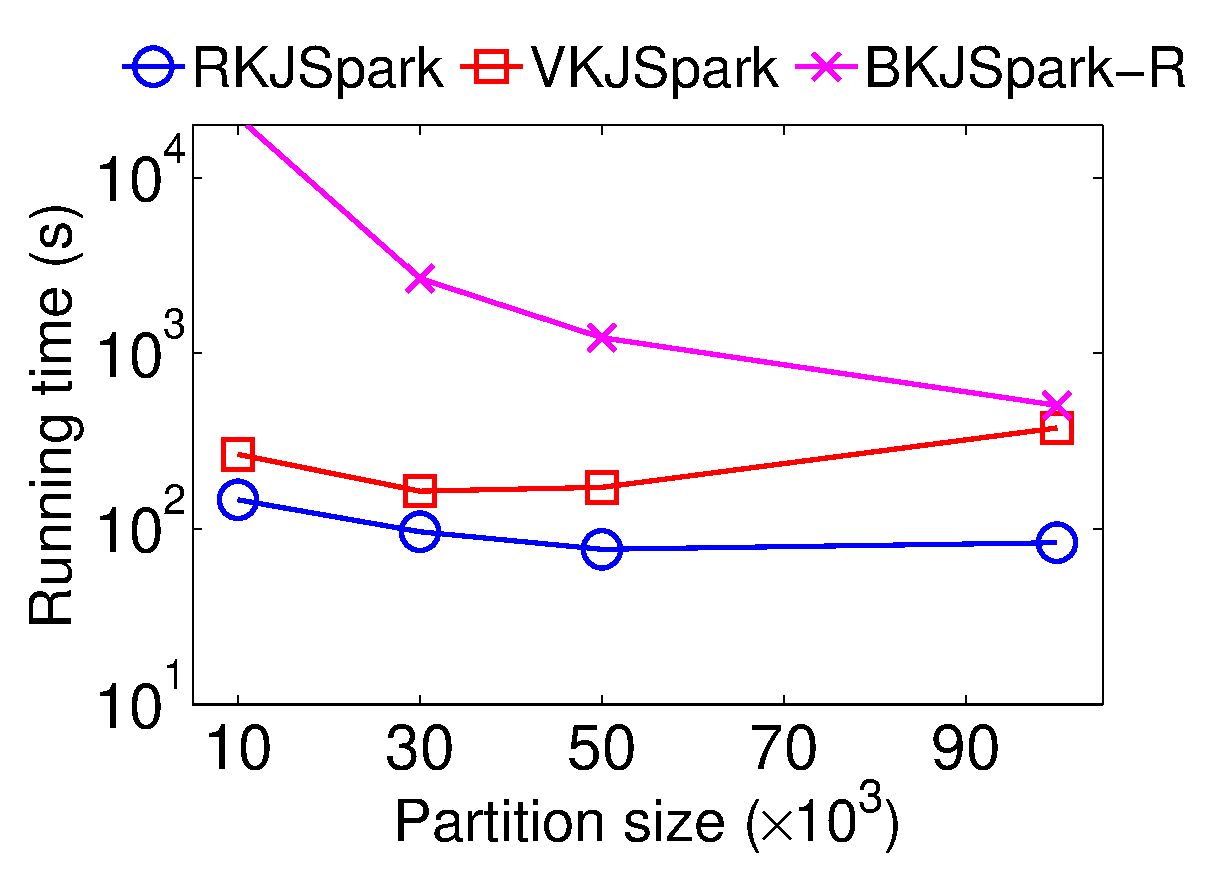
\includegraphics[width=1.55in]{figs/exp/osm_knnj_partsize}
  }
	\caption{Effect of partition size for join operations.}\vspace{-2mm}
	\label{fig:partsize_on_join}
\end{figure}

Figure \ref{fig:osm_knnj_partsize} presents how partition size effect
the performance of different $k$NN join approaches. With the increase
of partition size, BKJSpark-R and RKJSpark grow faster since fewer
local join tasks are required for join processing. VKJSpark becomes
slightly slower as the partition size increases because the power of
its distance pruning bounds weakens when the number of pivots decreases.


\begin{figure}[h!]
	\centering
	\subfigure[Throughput] {
		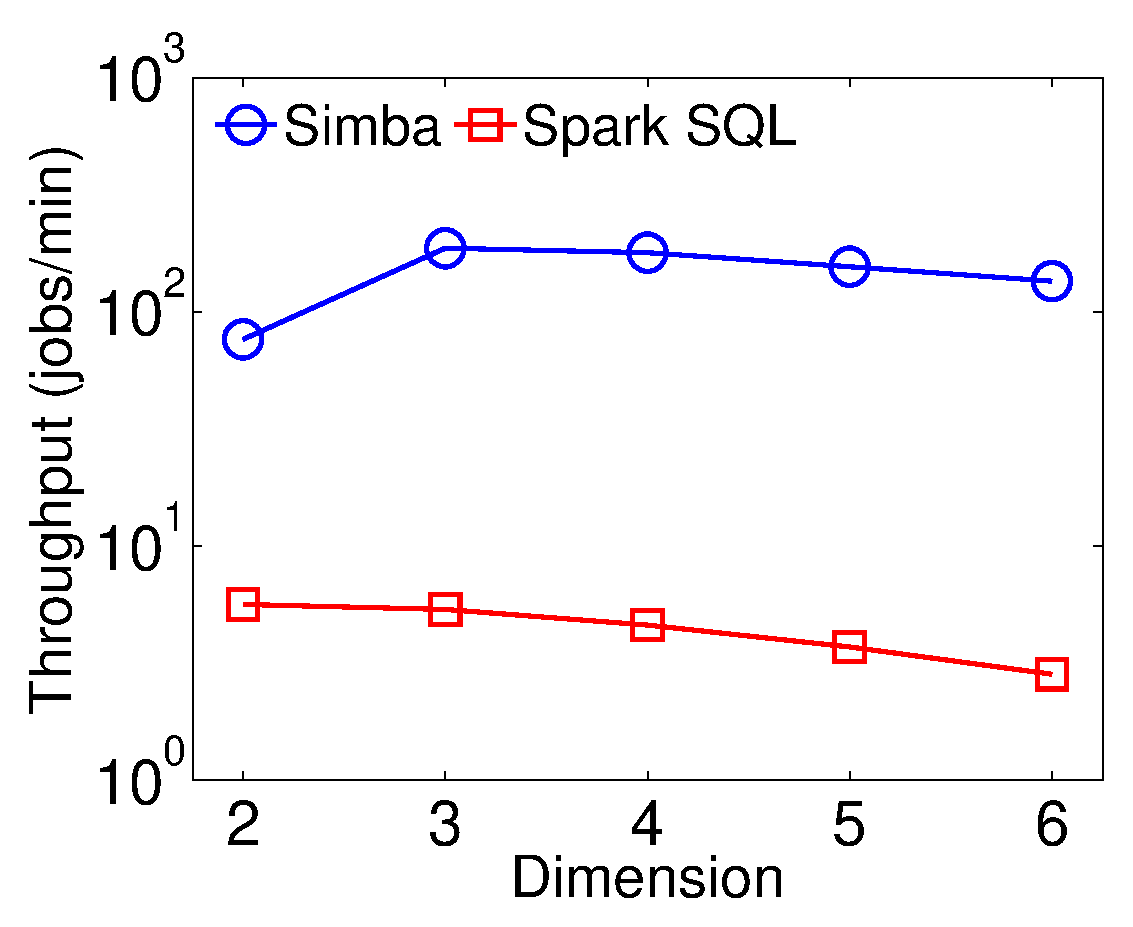
\includegraphics[width=1.55in]{figs/exp/gaussian700m_rect_dimension_throughput}
		\label{fig:rc_rect_dim_throughput}
	}
	\subfigure[Latency] {
		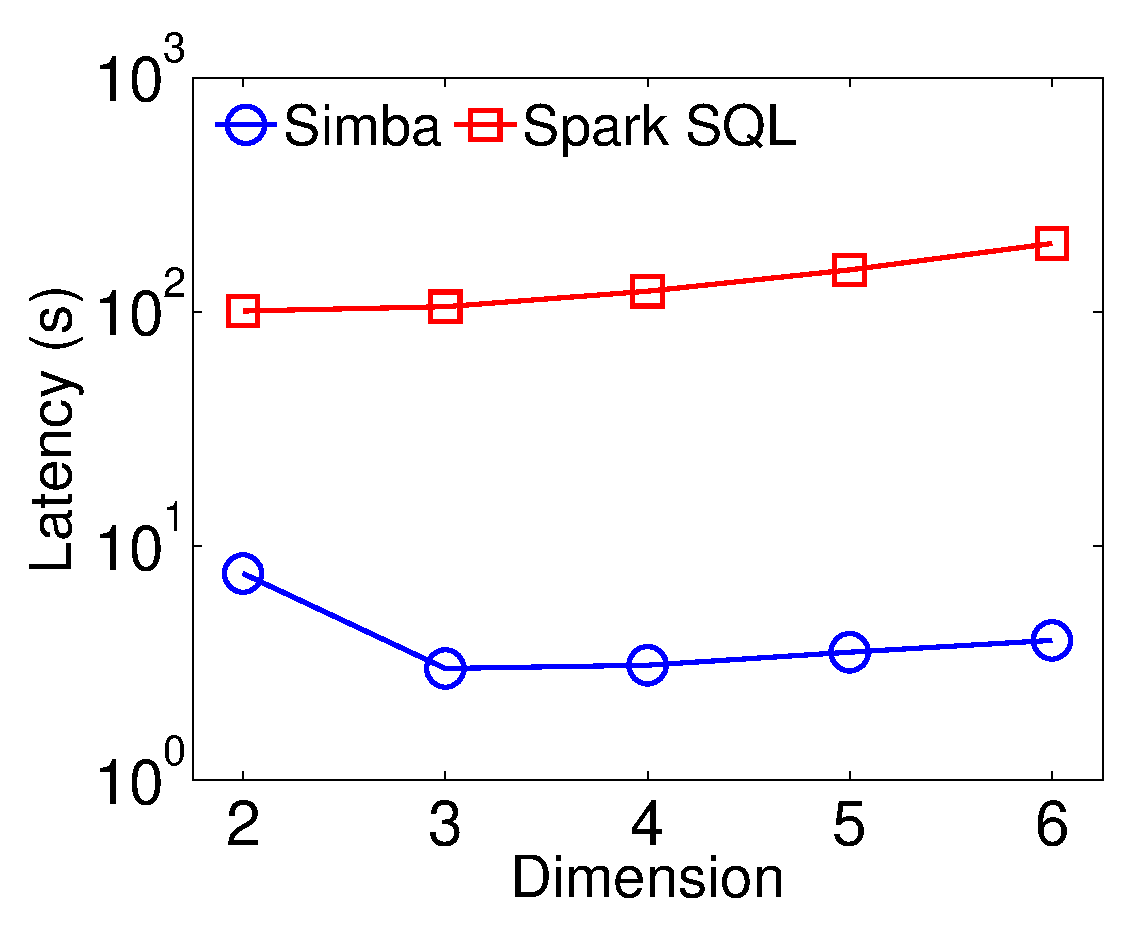
\includegraphics[width=1.55in]{figs/exp/gaussian700m_rect_dimension_latency}
		\label{fig:rc_rect_dim_latency}
	}
	\caption{\small Range query performance vs. dimensionality on RC.}
	\label{fig:rc_rect_dimension} %\vspace{-2mm}
\end{figure}

\begin{figure}[h!]
	\centering
	\subfigure[Throughput] {
		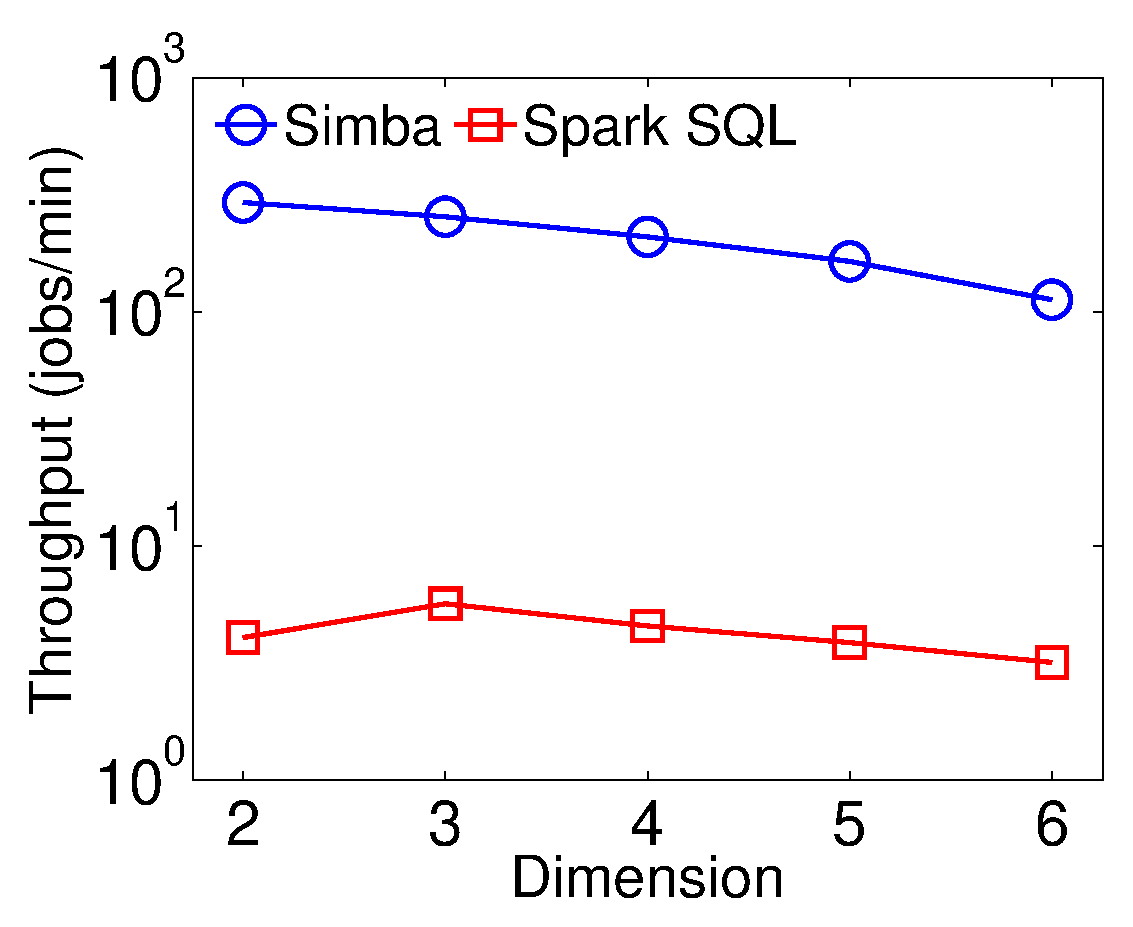
\includegraphics[width=1.55in]{figs/exp/gaussian700m_knn_dimension_throughput}
		\label{fig:rc_knn_dim_throughput}
	}
	\subfigure[Latency] {
		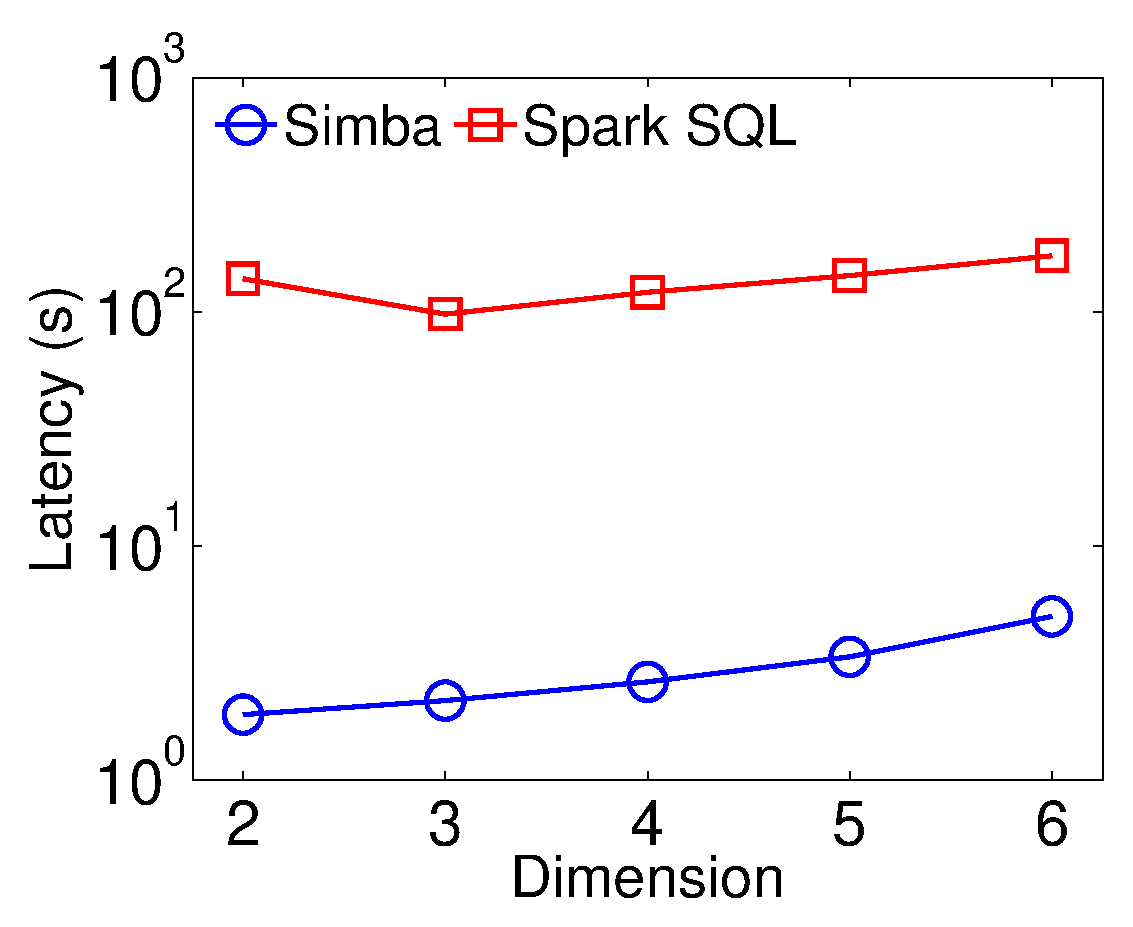
\includegraphics[width=1.55in]{figs/exp/gaussian700m_knn_dimension_latency}
		\label{fig:rc_knn_dim_latency}
	}
	\caption{\small $k$NN query performance vs. dimensionality on RC.}
	\label{fig:rc_knn_dimension} %\vspace{-2mm}
\end{figure}
Lastly, Figures \ref{fig:rc_rect_dimension} and \ref{fig:rc_knn_dimension}
show the results for range and $k$NN queries when dimensionality
increases from $2$ to $6$, using the synthetic RC data set. The
results show similar trends to that on the GEDLT dat set as in Figures
\ref{fig:gdelt_rect_dimension} and \ref{fig:gdelt_knn_dimension}: \name has significantly
outformed Spark SQL in all dimensions.

\end{appendix}
%%% Local Variables:
%%% mode: latex
%%% TeX-master: "paper"
%%% End:
